\newcommand{\fileInfectorTagResultsAucTable}{
    \begin{table}[H]
        \centering
        \begin{tabular}{|p{2,8cm}||p{2,8cm} p{2,8cm} p{2,8cm}|}
            \hline
            File-infector Tag & ALOHA & Joint Embedding & Proposed Model \\
            \hline
            AUC-ROC & 0.982$\pm$0.002 & 0.982$\pm$0.001 & \textBF{0.986$\pm$0.001} \\
            \hline
        \end{tabular}
        \caption{AUC-ROC (Area Under Curve) of the different models for the \textbf{File-infector Tag} prediction task. Results were aggregated over \textBF{3} training runs with different weight initializations and minibatch orderings. Best results are shown in \textbf{bold}.} \label{tab:fileInfectorTag_auc}
    \end{table}
}

\newcommand{\fileInfectorTagResultsAtFprTable}{
    \begin{center}
        \begin{longtable}[c]{|p{3,2cm}||p{1,8cm} p{1,8cm} p{1,8cm} p{1,8cm} p{1,8cm}|}
            \hline
            File-infector Tag & \multicolumn{5}{c|}{{FPR}} \\
            & $10^{-5}$ & $10^{-4}$ & $10^{-3}$ & $10^{-2}$ & $10^{-1}$ \\
            \hline
            \endfirsthead

            \caption*{\raggedright ...continued from previous page} \\
            \hline
            File-infector Tag & \multicolumn{5}{c|}{\textbf{FPR}} \\
            & $10^{-5}$ & $10^{-4}$ & $10^{-3}$ & $10^{-2}$ & $10^{-1}$ \\
            \hline
            \endhead

            \caption*{\raggedleft ...continued on next page} \\
            \endfoot

            \caption{Mean and standard deviation results (TPR, Accuracy, Recall, Precision and F1-Score) of the different models for the \textbf{File-infector Tag} prediction task at different \textbf{FPR}s (\textit{False Positive Rates}). Results were aggregated over \textBF{3} training runs with different weight initializations and minibatch orderings. Best results are shown in \textbf{bold}. Under \textbf{TPR} results are also presented the percentage reduction in mean detection error and in ROC curve standard deviation introduced by the \textit{Proposed Model} with respect to both \textit{ALOHA} model and \textit{Joint Embedding}.} \label{tab:fileInfectorTag_results_at_fpr} \\
            \endlastfoot

            \multicolumn{6}{|c|}{\textbf{TPR}} \\
            \hline
            ALOHA & 0.375$\pm$0.199 & 0.481$\pm$0.173 & 0.799$\pm$0.018 & 0.851$\pm$0.008 & 0.946$\pm$0.013 \\
            Joint Embedding & \textBF{0.433$\pm$0.157} & \textBF{0.558$\pm$0.115} & 0.791$\pm$0.028 & 0.862$\pm$0.009 & \textBF{0.959$\pm$0.002} \\
            Proposed Model & 0.365$\pm$0.193 & 0.507$\pm$0.152 & \textBF{0.841$\pm$0.025} & \textBF{0.876$\pm$0.003} & 0.945$\pm$0.003 \\
            \hline
            Error Reduction wrt \newline ALOHA & -1.6\% & 5.0\% & 20.9\% & 16.8\% & -1.9\% \\
            Error Reduction wrt \newline Joint Embedding & -12.0\% & -11.5\% & 23.9\% & 10.1\% & -34.1\% \\
            \hline
            Std Reduction wrt \newline ALOHA & 3.0\% & 12.1\% & -38.9\% & 62.5\% & 76.9\% \\
            Std Reduction wrt \newline Joint Embedding & -22.9\% & -32.2\% & 10.7\% & 66.7\% & -50.0\% \\
            \hline
            \multicolumn{6}{|c|}{\textbf{Accuracy}} \\
            \hline
            ALOHA & 0.899$\pm$0.032 & 0.916$\pm$0.028 & 0.967$\pm$0.003 & 0.968$\pm$0.001 & 0.907$\pm$0.002 \\
            Joint Embedding & \textBF{0.908$\pm$0.025} & \textBF{0.928$\pm$0.019} & 0.965$\pm$0.005 & 0.969$\pm$0.002 & \textBF{0.910$\pm$0.000} \\
            Proposed Model & 0.897$\pm$0.031 & 0.920$\pm$0.025 & \textBF{0.973$\pm$0.004} & \textBF{0.972$\pm$0.001} & 0.907$\pm$0.001 \\
            \hline
            \multicolumn{6}{|c|}{\textbf{Recall}} \\
            \hline
            ALOHA & 0.374$\pm$0.199 & 0.481$\pm$0.173 & 0.799$\pm$0.018 & 0.851$\pm$0.008 & 0.946$\pm$0.013 \\
            Joint Embedding & \textBF{0.433$\pm$0.157} & \textBF{0.558$\pm$0.115} & 0.791$\pm$0.028 & 0.862$\pm$0.009 & \textBF{0.959$\pm$0.002} \\
            Proposed Model & 0.364$\pm$0.194 & 0.507$\pm$0.152 & \textBF{0.841$\pm$0.025} & \textBF{0.876$\pm$0.003} & 0.945$\pm$0.003 \\
            \hline
            \multicolumn{6}{|c|}{\textbf{Precision}} \\
            \hline
            ALOHA & \textBF{1.000$\pm$0.000} & \textBF{0.999$\pm$0.000} & \textBF{0.994$\pm$0.000} & 0.943$\pm$0.000 & 0.646$\pm$0.003 \\
            Joint Embedding & \textBF{1.000$\pm$0.000} & \textBF{0.999$\pm$0.000} & 0.993$\pm$0.000 & 0.943$\pm$0.001 & \textBF{0.649$\pm$0.001} \\
            Proposed Model & \textBF{1.000$\pm$0.000} & \textBF{0.999$\pm$0.000} & \textBF{0.994$\pm$0.000} & \textBF{0.944$\pm$0.000} & 0.645$\pm$0.001 \\
            \hline
            \multicolumn{6}{|c|}{\textbf{F1 Score}} \\
            \hline
            ALOHA & 0.517$\pm$0.195 & 0.632$\pm$0.150 & 0.886$\pm$0.011 & 0.894$\pm$0.004 & 0.767$\pm$0.006 \\
            Joint Embedding & \textBF{0.588$\pm$0.154} & \textBF{0.709$\pm$0.093} & 0.881$\pm$0.017 & 0.901$\pm$0.005 & \textBF{0.774$\pm$0.001} \\
            Proposed Model & 0.500$\pm$0.237 & 0.658$\pm$0.144 & \textBF{0.911$\pm$0.015} & \textBF{0.909$\pm$0.002} & 0.767$\pm$0.002 \\
            \hline
        \end{longtable}
    \end{center}
}

\newcommand{\fileInfectorTagResultsSummaryTable}{
    \begin{table}[H]
        \centering
        \begin{tabular}{|p{3,2cm}||p{1,8cm} p{1,8cm} p{1,8cm} p{1,8cm} p{1,8cm}|}
            \hline
            \multicolumn{6}{|c|}{File-infector Tag (at FPR $=1\%$)} \\
            \hline
            Model & TPR & Accuracy & Precision & Recall & F1 score \\
            \hline
            ALOHA & 0.851$\pm$0.008 & 0.968$\pm$0.001 & 0.943$\pm$0.000 & 0.851$\pm$0.008 & 0.894$\pm$0.004 \\
            Joint Embedding & 0.862$\pm$0.009 & 0.969$\pm$0.002 & 0.943$\pm$0.001 & 0.862$\pm$0.009 & 0.901$\pm$0.005 \\
            Proposed Model & \textBF{0.876$\pm$0.003} & \textBF{0.972$\pm$0.001} & \textBF{0.944$\pm$0.000} & \textBF{0.876$\pm$0.003} & \textBF{0.909$\pm$0.002} \\
            \hline
        \end{tabular}
        \caption{Summary of the mean and standard deviation results of the different models for the \textbf{File-infector Tag} prediction task at \textbf{FPR} $=1\%$. Results were aggregated over \textBF{3} training runs with different weight initializations and minibatch orderings. Best results are shown in \textbf{bold}.} \label{tab:fileInfectorTag_result_summary}
    \end{table}
}

\newcommand{\fileInfectorTagRocAloha}{
    \begin{figure}[H]
        \vspace*{-0.5cm}
        \centering
        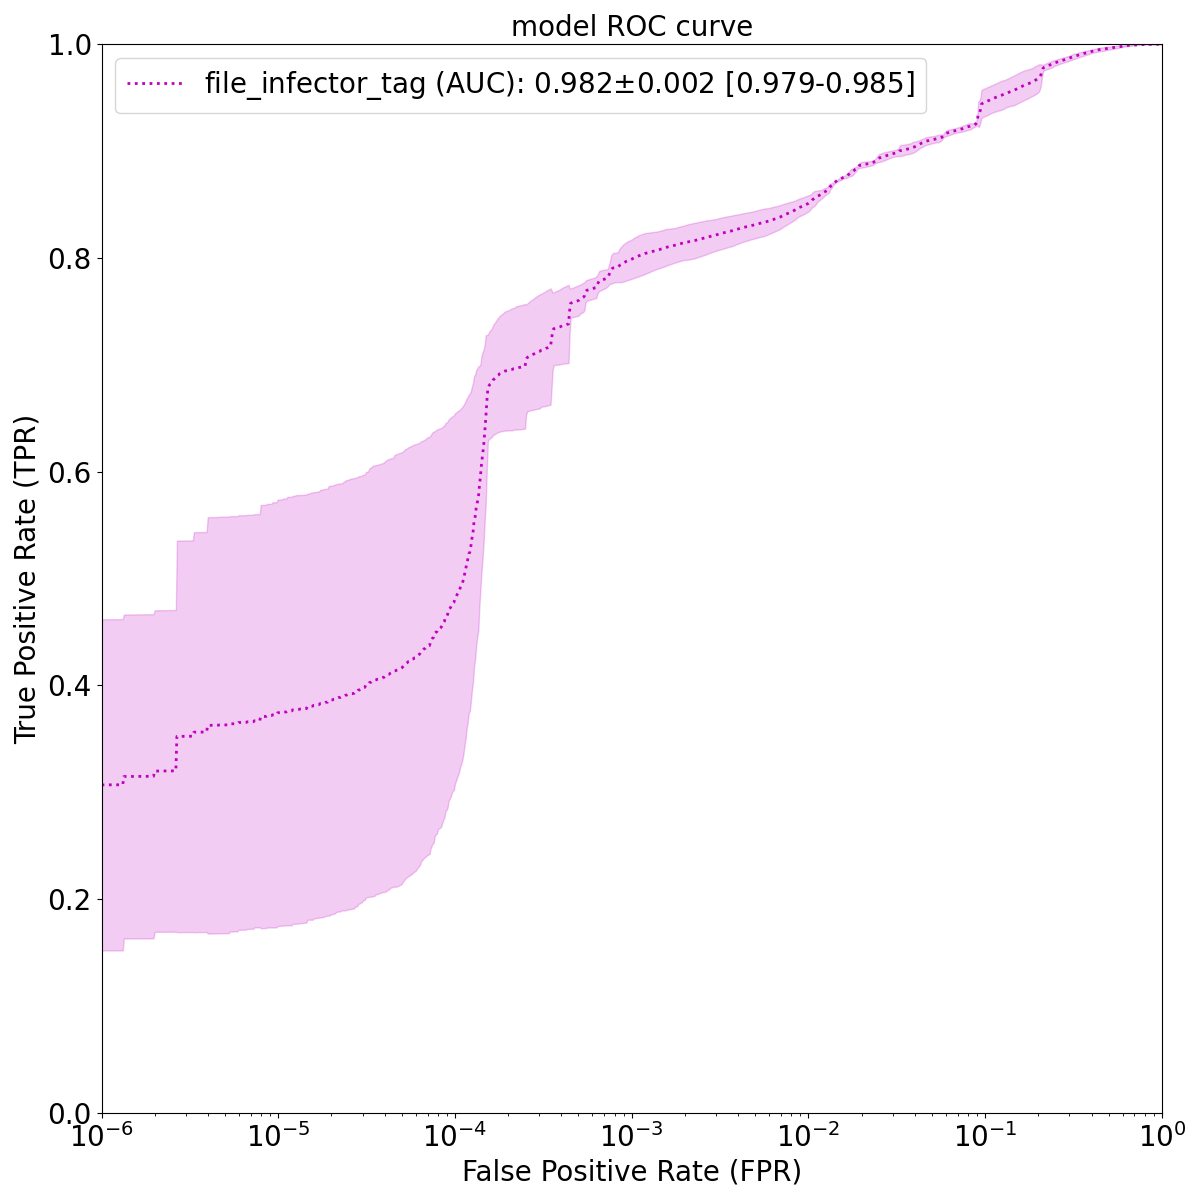
\includegraphics[width=0.6\textwidth]{./results/file_infector_tag_roc_aloha.png}
        \vspace*{-0.2cm}
        \caption{ROC curve and AUC statistics of \textBF{ALOHA} model for the \textbf{File-infector Tag}. The line represents the \textit{mean} TPR at a given FPR, while the shaded region represents the \textit{standard deviation}. Statistics were computed over \textBF{3} training runs, each with random parameter initialization.}
        \label{fig:fileInfectorTagRocAloha}
    \end{figure}
}

\newcommand{\fileInfectorTagRocJointEmbedding}{
    \begin{figure}[H]
        \vspace*{-0.5cm}
        \centering
        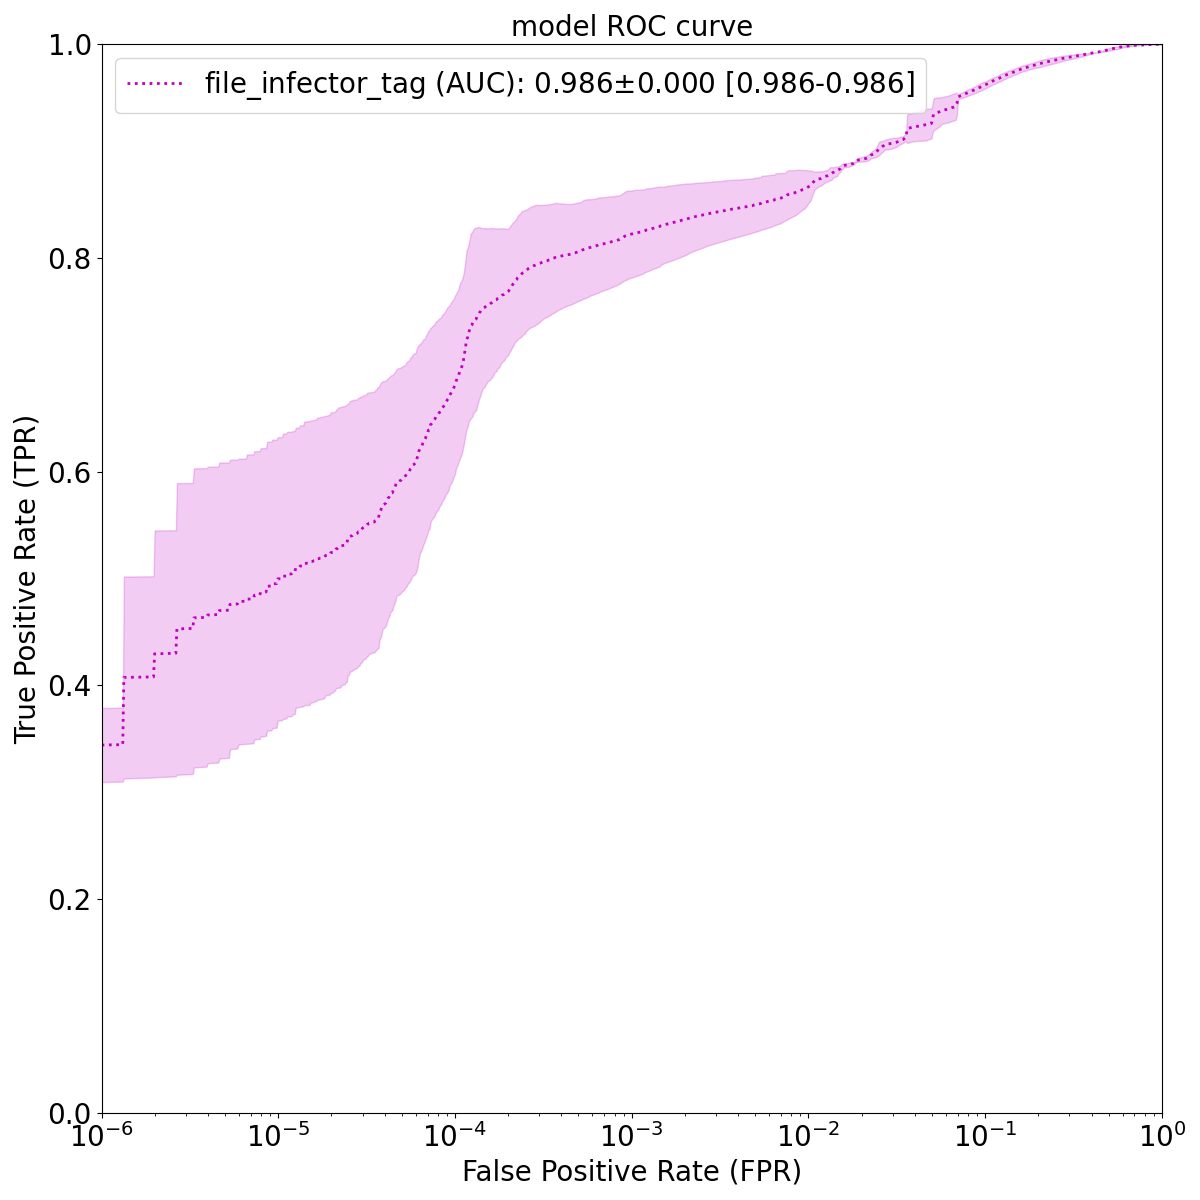
\includegraphics[width=0.6\textwidth]{./results/file_infector_tag_roc_jointEmbedding.png}
        \vspace*{-0.2cm}
        \caption{ROC curve and AUC statistics of \textBF{Joint Embedding} model for the \textbf{File-infector Tag}. The line represents the \textit{mean} TPR at a given FPR, while the shaded region represents the \textit{standard deviation}. Statistics were computed over \textBF{3} training runs, each with random parameter initialization.}
        \label{fig:fileInfectorTagRocJointEmbedding}
    \end{figure}
}

\newcommand{\fileInfectorTagRocProposedMethod}{
    \begin{figure}[H]
        \vspace*{-0.5cm}
        \centering
        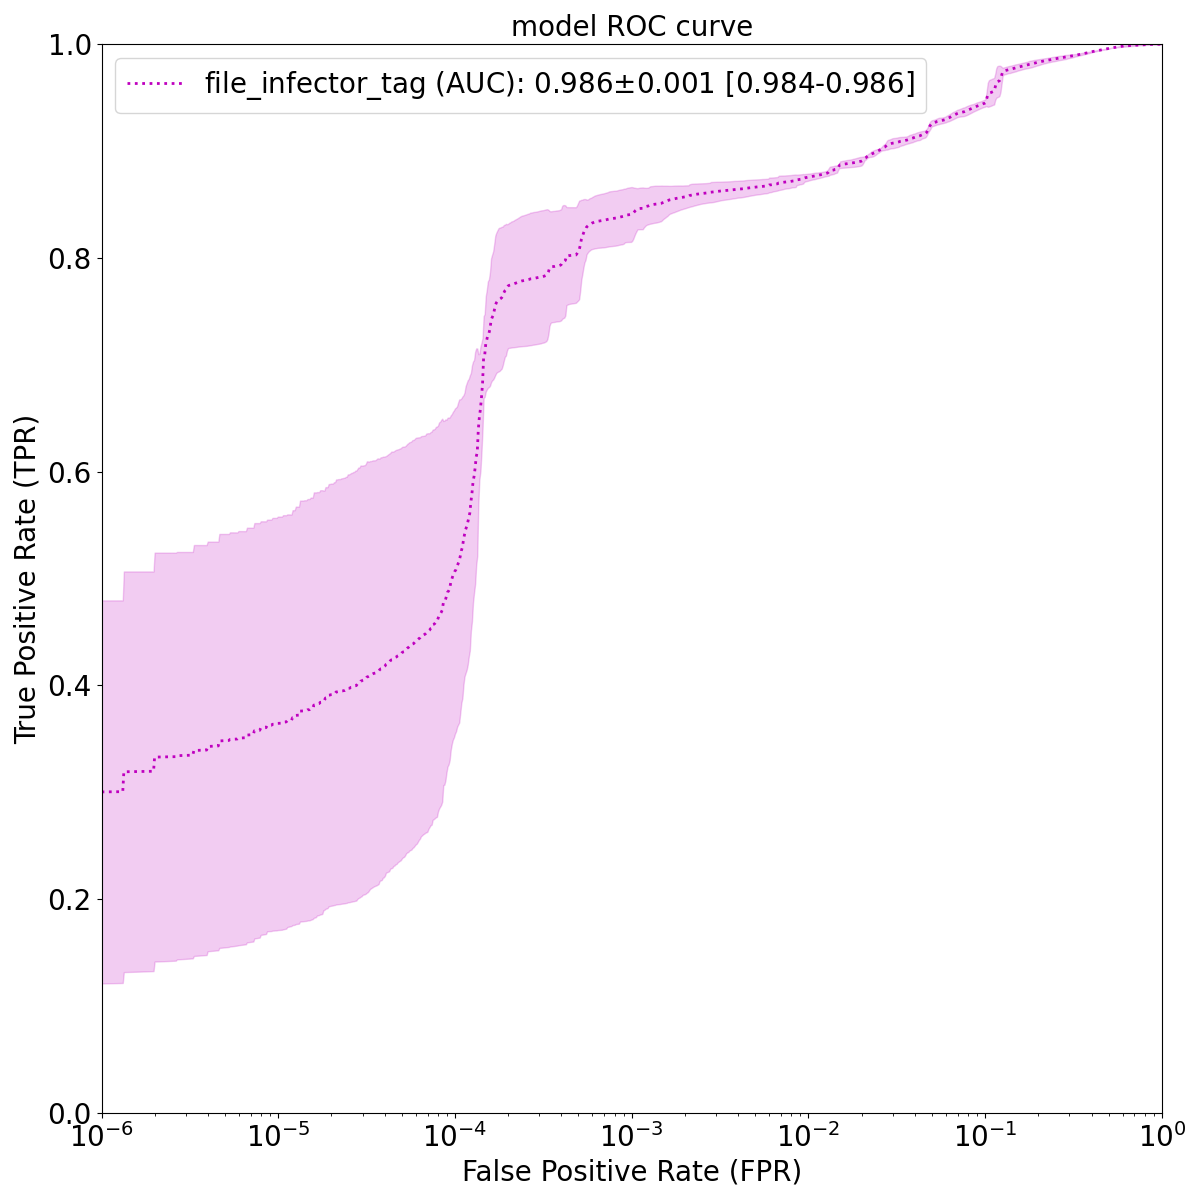
\includegraphics[width=0.6\textwidth]{./results/file_infector_tag_roc_proposedModel.png}
        \vspace*{-0.2cm}
        \caption{ROC curve and AUC statistics of \textBF{Proposed Model} for the \textbf{File-infector Tag}. The line represents the \textit{mean} TPR at a given FPR, while the shaded region represents the \textit{standard deviation}. Statistics were computed over \textBF{3} training runs, each with random parameter initialization.}
        \label{fig:fileInfectorTagRocProposedModel}
    \end{figure}
}
